
\begin{frame}[fragile]{Machine code}

  \begin{itemize}
    \tightlist
  \item
    Detailed instructions for the actions of the CPU
  \item
    Not human readable
  \item
    Sample types of instructions:

    \begin{itemize}
      \tightlist
    \item
      Transfer data between memory location and register
    \item
      Perform arithmetic/logic operations with data in register
    \item
      Check if data in register fulfills some condition
    \item
      Conditionally change the memory address from where instructions are
      fetched \(~\equiv~\) ``jump'' to address
    \item
      Save all register context and take instructions from different
      memory location until return \(~\equiv~\) ``call''
    \end{itemize}

  \item Instructions are very hard to handle, although programming 
    started this way $\dots$

    \begin{textcode}
      534c 29e5 31db 48c1 fd03 4883 ec08 e85d 
      feff ff48 85ed 741e 0f1f 8400 0000 0000 
      4c89 ea4c 89f6 4489 ff41 ff14 dc48 83c3 
      0148 39eb 75ea 4883 c408 5b5d 415c 415d 
      415e 415f c390 662e 0f1f 8400 0000 0000 
      f3c3 0000 4883 ec08 4883 c408 c300 0000 
      0100 0200 4865 6c6c 6f20 776f 726c 6400 
      011b 033b 3400 0000 0500 0000 20fe ffff 
      8000 0000 60fe ffff 5000 0000 4dff ffff 
    \end{textcode}
  \end{itemize}

\end{frame}

\begin{frame}[fragile]{Assembler code}

  \begin{itemize}
    \tightlist
  \item
    Human readable representation of CPU instructions
  \item
    Some write it by hand \ldots{}

    \begin{itemize}
      \tightlist
    \item
      Code close to abilities and structure of the machine
    \item
      Handle constrained resources (embedded systems, early computers)
    \end{itemize}
  \item
    Translated to machine code by a programm called \emph{assembler}
  \end{itemize}

  \begin{textcode}
    .file   "code.c"
    .section    .rodata
    .LC0:
    .string "Hello world"
    .text
    ...
    pushq   %rbp
    .cfi_def_cfa_offset 16
    .cfi_offset 6, -16
    movq    %rsp, %rbp
    .cfi_def_cfa_register 6
    subq    $16, %rsp
    movl    %edi, -4(%rbp)
    movq    %rsi, -16(%rbp)
    movl    $.LC0, %edi
    movl    $0, %eax
    call    printf
  \end{textcode}

\end{frame}

\begin{frame}[fragile]{Compiled high level languages}

  \begin{itemize}
    \tightlist
  \item
    Algorithm description using mix of mathematical formulas and
    statements inspired by human language
  \item
    Translated to machine code (resp. assembler) by \emph{compiler}
  \end{itemize}

  \begin{ccode}
    #include <stdio.h>
    int main (int argc, char *argv[])
    {
      printf("Hello world"); 
    }
  \end{ccode}

  \begin{itemize}
    \tightlist
  \item
    ``Far away'' from CPU \(~\Rightarrow\) the compiler is responsible for
    creation of optimized machine code
  \item
    Fortran, COBOL, C, Pascal, Ada, Modula2, C++, Go, Rust, Swift
  \item
    Strongly typed
  \item
    Tedious workflow: compile - link - run
  \end{itemize}

  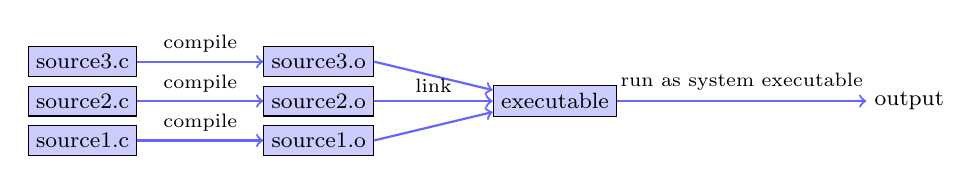
\begin{tikzpicture}
    {\footnotesize
      \node(s3) at (0,1.0) [fill=blue!20,draw] {source3.c};
      \node(s2) at (0,0.5) [fill=blue!20,draw] {source2.c};
      \node(s1) at (0,0.0) [fill=blue!20,draw] {source1.c};
      
      \node(o3) at (3,1.0) [fill=blue!20,draw] {source3.o};
      \node(o2) at (3,0.5) [fill=blue!20,draw] {source2.o};
      \node(o1) at (3,0.0) [fill=blue!20,draw] {source1.o};
      
      \node(x) at (6,0.5) [fill=blue!20,draw]  {executable};

      \node(out) at (10.5,0.5) {output};

      \draw (s3.east) edge[->, blue!60, thick] node[above,black]{\scriptsize compile} (o3.west);
      \draw (s2.east) edge[->, blue!60, thick] node[above,black]{\scriptsize compile} (o2.west);
      \draw (s1.east) edge[->, blue!60, thick] node[above,black]{\scriptsize compile} (o1.west);

      \draw (o3.east) edge[->, blue!60, thick]  (x.170); 
      \draw (o2.east) edge[->, blue!60, thick] node[above,black]{\scriptsize link} (x.180); }
    \draw (o1.east) edge[->, blue!60, thick]  (x.190);

    \draw (x.east) edge[->, blue!60, thick]  node[above,black]{\scriptsize run as system executable} (out.west);
  \end{tikzpicture}

\end{frame}


\only<beamer>{
  \begin{frame}{Compiling\ldots{}}

    \begin{center}
      \includegraphics[width=0.8\textwidth]{pic/compiling}
    \end{center}

    \ldots{} from xkcd

  \end{frame}
}

\begin{frame}{Compiled languages in Scientific Computing}

  \begin{itemize}
    \tightlist
  \item
    Fortran: FORmula TRANslator (1957)

    \begin{itemize}
      \tightlist
    \item
      Fortran4: really dead
    \item
      Fortran77: large number of legacy libs: BLAS, LAPACK, ARPACK
      \ldots{}
    \item
      Fortran90, Fortran2003, Fortran 2008

      \begin{itemize}
        \tightlist
      \item
        Catch up with features of C/C++
        (structures,allocation,classes,inheritance, C/C++ library calls)
      \item
        Lost momentum among new programmers
      \item
        Hard to integrate with C/C++
      \item
        In many aspects very well adapted to numerical computing
      \item
        Well designed multidimensional arrays
      \end{itemize}
    \end{itemize}
  \item
    C: General purpose language

    \begin{itemize}
      \tightlist
    \item
      K\&R C (1978) weak type checking
    \item
      ANSI C (1989) strong type checking
    \item
      Had structures and allocation early on
    \item
      Numerical methods support via libraries
    \item
      Fortran library calls possible
    \end{itemize}
  \item
    C++: \emph{The} powerful object oriented language

    \begin{itemize}
      \tightlist
    \item
      Superset of C (in a first approximation)
    \item
      Classes, inheritance, overloading, templates (generic programming)
    \item
      C++11: $\approx 2011$ Quantum leap: smart pointers, threads, lambdas, initializer
      lists in standard
    \item Since then: C++14, C++17, C++20
    \item
      With great power comes the possibility of great failure\ldots{}
    \end{itemize}
  \end{itemize}

\end{frame}

\begin{frame}[fragile]{High level scripting languages}

  \begin{itemize}
    \tightlist
  \item
    Algorithm description using mix of mathematical formulas and
    statements inspired by human language
  \item 
    Simpler syntax, less "boiler plate"
  \end{itemize}

  \begin{pythoncode}
    print("Hello world")
  \end{pythoncode}

  \begin{itemize}
    \tightlist
  \item
    Need intepreter in order to be executed
  \item
    Very far away from CPU \(~\Rightarrow\) usually significantly slower
    compared to compiled languages
  \item
    Matlab, Python, Lua, perl, R, Java, javascript
  \item
    Less strict type checking, powerful introspection
    capabilities
  \item
    Immediate workflow: ``just run''

    \begin{itemize}
      \tightlist
    \item
      in fact: first compiled to \emph{bytecode} which can be interpreted
      more efficiently
    \end{itemize}
  \end{itemize}

  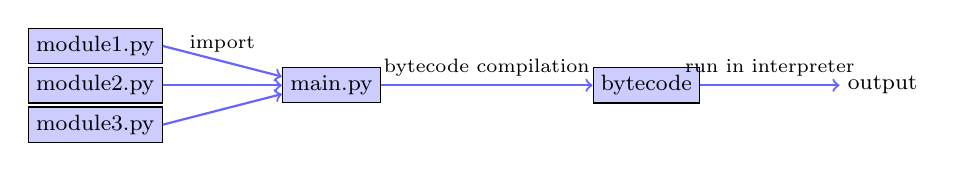
\begin{tikzpicture}
    {\footnotesize
      \node(s3) at (3,1.0) [fill=blue!20,draw] {module1.py};
      \node(s2) at (3,0.5) [fill=blue!20,draw] {module2.py};
      \node(s1) at (3,0.0) [fill=blue!20,draw] {module3.py};

      \node(x) at (6,0.5) [fill=blue!20,draw]  {main.py};


      \node(b) at (10,0.5) [fill=blue!20,draw]  {bytecode};

      \node(out) at (13,0.5) {output};


      \draw (s3.east) edge[->, blue!60, thick] node[above,black]{\scriptsize import}  (x.170); 
      \draw (s2.east) edge[->, blue!60, thick] (x.180); 
    \draw (s1.east) edge[->, blue!60, thick]  (x.190);
    \draw (x.east) edge[->, blue!60, thick]  node[above,black]{\scriptsize bytecode compilation} (b.west);

    \draw (b.east) edge[->, blue!60, thick]  node[above,black]{\scriptsize run in interpreter} (out.west);
    }
  \end{tikzpicture}

\end{frame}

\begin{frame}{JIT based languages}

  \begin{itemize}
    \tightlist
  \item
    Most interpreted language first compile to
    bytecode wich then is run in the interpreter and not on the processor $\Rightarrow$ perfomance bottleneck,
    \begin{itemize}
      \tightlist
    \item  remedy: use compiled language  for performance critical parts
    \item  ``two language problem'', additional work for interface code
    \end{itemize}
  \item Better: Just In Time compiler (JIT): compile to machine code ``on the fly''
    \begin{itemize}
      \tightlist
    \item
      V8 \(~\to\) javascript
    \item
      LuaJIT, Java, Smalltalk
    \item   LLVM    \(~\to\)   \textbf{Julia} (v1.0 since August, 2018)
    \item
      LLVM Compiler infrastructure \(~\to\) Python/NUMBA
    \end{itemize}
  \item
    Drawback over compiled languages: compilation delay at every start,
    can be mediated by caching
  \item
    Advantage over compiled languages: simpler syntax, \emph{tracing} JIT,
    i.e.~optimization at runtime
\end{itemize}
\vfill

  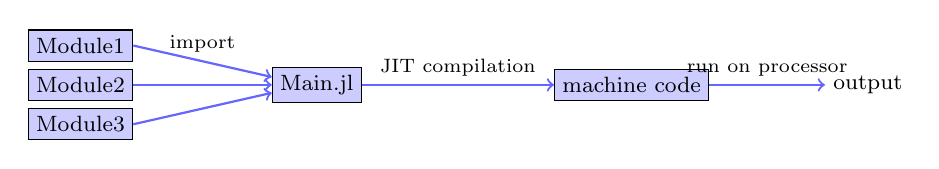
\begin{tikzpicture}
    {\footnotesize
      \node(s3) at (3,1.0) [fill=blue!20,draw] {Module1};
      \node(s2) at (3,0.5) [fill=blue!20,draw] {Module2};
      \node(s1) at (3,0.0) [fill=blue!20,draw] {Module3};

      \node(x) at (6,0.5) [fill=blue!20,draw]  {Main.jl};


      \node(b) at (10,0.5) [fill=blue!20,draw]  {machine code};

      \node(out) at (13,0.5) {output};


      \draw (s3.east) edge[->, blue!60, thick] node[above,black]{\scriptsize import}  (x.170); 
      \draw (s2.east) edge[->, blue!60, thick] (x.180); 
    \draw (s1.east) edge[->, blue!60, thick]  (x.190);
    \draw (x.east) edge[->, blue!60, thick]  node[above,black]{\scriptsize JIT compilation} (b.west);

    \draw (b.east) edge[->, blue!60, thick]  node[above,black]{\scriptsize run on processor} (out.west);
    }
  \end{tikzpicture}


\end{frame}


\begin{frame}\frametitle{Julia History \& Resources}
  \begin{columns}
    \begin{column}{0.6\textwidth}
  \begin{itemize}
  \item 2009-02:  V0.1 Development started in 2009 at MIT (S. Bezanson, S. Karpinski, V. Shah, A. Edelman)
    
  \item    2012: V0.1
    
  \item 2016-10: V0.5 experimental threading support
  \item 2017-02: SIAM Review: Julia - A Fresh Approach to Numerical Computing
  \item 2018-08: \textbf{V1.0}
  \item 2018 Wilkinson Prize for numerical software
  \end{itemize}

    \end{column}
    \begin{column}{0.4\textwidth}
      \begin{center}
        \includegraphics[width=0.5\textwidth]{julia}
        \includegraphics[width=\textwidth]{julia-langauge-developers-mit-00_0}      
      \end{center}
    \end{column}
  \end{columns}

  \vfill
  \begin{itemize}
  \item Homepage incl. download link: \url{https://julialang.org/}
  \item Wikibook: \url{https://en.wikibooks.org/wiki/Introducing_Julia}
  \item TU Berlin Jupyter server \url{https://www-pool.math.tu-berlin.de/jupyter}: you will
    be able to user your UNIX pool account
  \end{itemize}


\end{frame}
%%%%%%%%%%%%%%%%%%%%%%%%%%%%%%%%%%%%%%%%%%%%%%%%%%%%%%%%%%%%%%%%%%%%%%%%%%%%%% 


%%%%%%%%%%%%%%%%%%%%%%%%%%%%%%%%%%%%%%%%%%%%%%%%%%%%%%%%%%%%%%%%%%%%%%%%%%%%%% 
\begin{frame}\frametitle{Julia - a first characterization}
``\textbf{Like matlab, but faster}''

``\textbf{Like matlab, but open source}''

``\textbf{Like python + numpy, but faster and counting from 1}''

  \begin{itemize}
  \item Main purpose: performant numerics 
  \item Multidimensional arrays as first class objects\\
    (like Fortran, Matlab; unlike C++, Swift, Rust, Go $\dots$)
  \item  Array indices counting from 1\\ (like Fortran, Matlab; unlike C++, python) - but it seems this becomes
    more flexible
  \item Array slicing etc.
  \item Extensive library of standard functions, linear algebra operations
  \item Package ecosystem
  \end{itemize}
\end{frame}
%%%%%%%%%%%%%%%%%%%%%%%%%%%%%%%%%%%%%%%%%%%%%%%%%%%%%%%%%%%%%%%%%%%%%%%%%%%%%% 

%%%%%%%%%%%%%%%%%%%%%%%%%%%%%%%%%%%%%%%%%%%%%%%%%%%%%%%%%%%%%%%%%%%%%%%%%%%%%% 
\begin{frame}\frametitle{$\dots$ there is more to the picture}
  \begin{itemize}
  \item Developed from scratch using modern knowledge in language development
  \item Strongly typed $\Rightarrow$ JIT compilation to performant code
  \item Multiple dispatch: all functions are essentialy templates
  \item Parallelization: SIMD, threading, distributed  memory
  \item Reflexive: one can loop over struct elements
  \item Module system, module precompilation
  \item REPL (Read-Eval-Print-Loop)
    
  \item Ecosystem:
    \begin{itemize}
    \item Package manager with github integration
    \item Foreign function interface to C, Fortran, wrapper methods for  C++
    \item PyCall.jl: loading of python modules via reflexive proxy objects (e.g. plotting)
    \item Intrinsic tools for documentation, profiling, testing
    \item Code inspection of LLVM and native assembler codes
    \item IDE integration e.g. via atom editor (Juno)
    \item Jupyter notebooks
    \end{itemize}
  \end{itemize}
\end{frame}
%%%%%%%%%%%%%%%%%%%%%%%%%%%%%%%%%%%%%%%%%%%%%%%%%%%%%%%%%%%%%%%%%%%%%%%%%%%%%% 



%%% Local Variables:
%%% mode: latex
%%% TeX-master: "l01-intro"
%%% End:
